% !TEX encoding = UTF-8 Unicode
%%
%%		XX_名前_日付.{tex,pdf}
%%		XX, 名前, 日付は naming rule に従う
%%
\documentclass[11pt,a4paper]{jsarticle}

%% ページ設定のパラメータは変更しない
\usepackage[top=72pt,bottom=60pt,left=40pt,right=40pt]{geometry}
\setlength{\topmargin}{-38pt}
\setlength{\headheight}{18pt}
\setlength{\headsep}{20pt}
\setlength{\footskip}{38pt}
\setlength{\topskip}{0pt}
%%

%% 共通フォーマット
\usepackage{fancyhdr}
\rhead{\stdid, \sirname}
\cfoot{}
\rfoot{\thepage}
\renewcommand{\footrulewidth}{\headrulewidth}
\pagestyle{fancy}

\usepackage{subfig}
\usepackage{layout}

%% \title{maketitleは使わない}
%% \author{}
%% \date{}

%% 自分の使うパッケージ
\usepackage{amsmath,amssymb}
\usepackage{bm}
\usepackage[dvipdfmx]{graphicx}
\usepackage{ascmac}
\usepackage{indentfirst}
\graphicspath{{./images/}}

%% 個人設定、日付設定
\lfoot{\today}		%% 日付
\def\stdid{18T0006}		%% 学生証番号
\def\sirname{小室}		%% 姓
\def\firstname{光広}		%% 名


\begin{document}
%% \maketitle			%% maketitle は使わない

\noindent
\textbf{\large 進捗レポート (\stdid, \sirname\ \firstname)}		%%  固定

%%
\section*{今週の進捗サマリ}			%% 固定

\begin{itemize}
\item テーマ再定義
\item 実装技術選定
\end{itemize}

%%
\section{進捗詳細}					%% 固定
\subsection{テーマ再設定}
従来より考えていたNLPタスクをベンチマークとするユーザー意図抽出モデル
(Part of Leica model)は収束が難しいと判断した.修士論文を執筆する
上で確実に時間が足りないと予想されるためである.したがって,本修士論文
で扱うテーマは,従来のNLPタスクではなく,より簡単な\texttt{Open AI
 Gym}環境における強化学習フレームワークの提案とする.\par
本研究では,従来の強化学習における局所解脱出性や,学習収束速度向上を目的
として,強化学習フレームワークにおけるAgentにDurable valueをもたせる
ことで試みる.本研究では以下に示す2つのモデルを設定した.
\begin{figure}[htbp]
  \begin{center}
    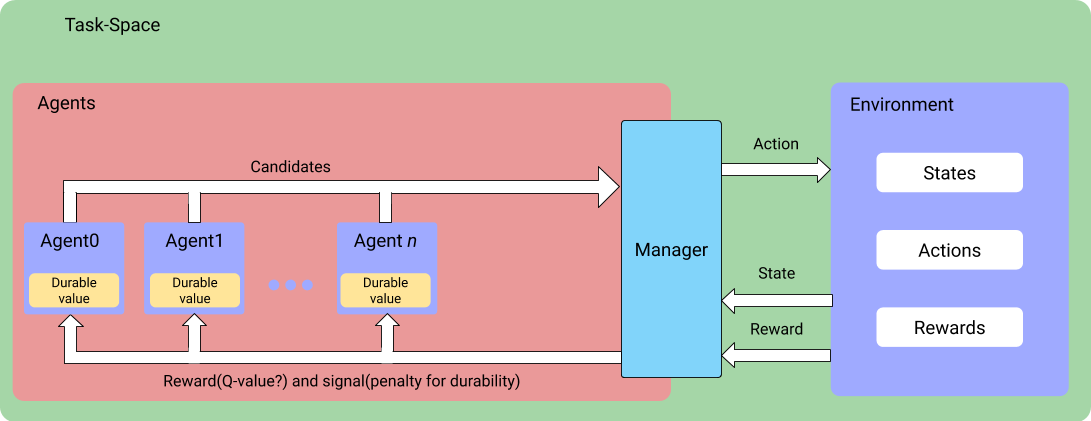
\includegraphics[width=14cm]{fig1.png}
    \caption{Syncモデル(仮称)}
  \end{center}
  \label{fig1}
\end{figure}
\begin{figure}[htbp]
  \begin{center}
    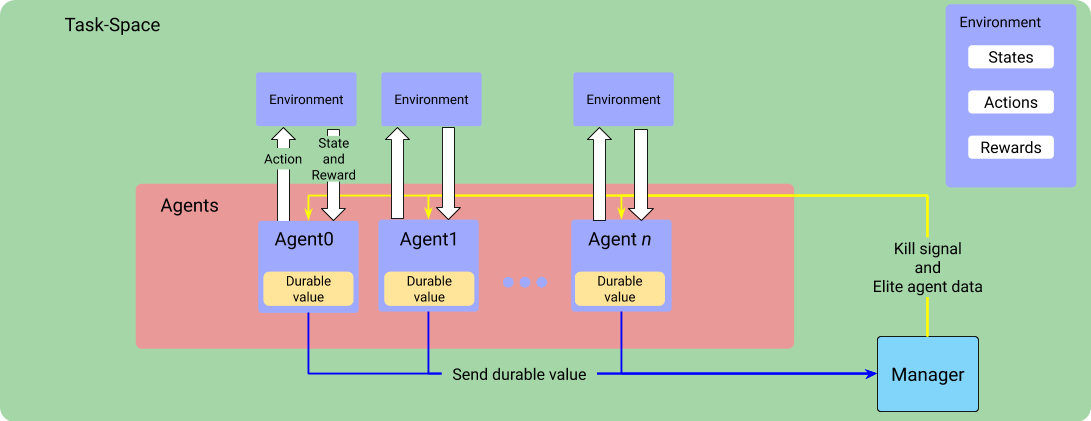
\includegraphics[width=14cm]{fig2.png}
    \caption{Asyncモデル(仮称)}
  \end{center}
  \label{fig2}
\end{figure}
本研究ではSyncモデルを始めに対象として扱い,時間があればAsyncモデルの検討
を行う.\par
以下,Syncモデルについて詳細を述べる.Syncモデルにおいて各AgentはDurable
valueを持っており,例えば\textbf{各エピソードで同じ動作をする}ことや,
\textbf{想定しない動作に収束する局所解状態を維持する}ことが見られた場合,その
Agentが持つDurable valueは減少する.ある閾値を超えて減少した場合そのAgentは
KillまたはSwapされる.Swapはその時点である評価手法で優秀と判断されたAgentの
オブジェクトをそのままコピーすることで実現する.\par
以上のSyncモデルにおいて,AgentはCNN等のニューラルネットワークを使用し,DQN
による\texttt{Open AI Gym Atari}によるゲームでその精度値を評価する.

\subsection{実装技術選定}
モデルを実装するに当たり,実装で必要となる以下のライブラリを調査した.
\begin{itemize}
  \item TF-agent
  \item keras-rl
  \item Chainer-rl
  \item PyTorch
\end{itemize}
まず\texttt{TF-agent}は\texttt{TensorFlow 2.0 bata}以降に追加となった
強化学習向けライブラリである.本ライブラリにEnvironment Suiteとして
\texttt{Open AI Gym}環境も含まれており,比較的扱いやすい(\texttt{TensorFlow
 1.13.x}以降Eager executionがデフォルトとなり,Sessionの概念が消えたため)ため
実装も比較的しやすいと考えられる.一方,ライブラリはbeta版であり,今後正式リリース時
に挙動が変化することも容易に考えられる.\par
次に\texttt{Keras-rl}である.このライブラリは\texttt{Keras}をベースとし,比較的
わかりやすいコードでネットワーク定義などができる.一方,本研究において必要となる学習
ループ中の処理について自前で実装する場合,\texttt{keras.model.fit()}によりラップ
されているため,ソースコードを読み,クラスを継承した上で実装しなければならず,時間的制約
が問題となる.\par
\texttt{Chainer-rl}は\texttt{Chainer}を強化学習向けに適用した新たなライブラリである.
国産機械学習ライブラリであり,文献等も多く存在するが,これも学習ループがラップされているため
実装上の時間的制約で断念した.\par
最後に\texttt{PyTorch}である.本ライブラリは本研究室井川氏の研究実装において使用された実績
があり,Facebookが作るOSS機械学習ライブラリである.本ライブラリでは学習ループを自前で用意する
必要があり,本研究実装に都合が良いと考えられる.加えて\texttt{TensorBoard}による可視化も対応
することからデータ分析が容易になるという利点もある.\par
以上より,本研究では\texttt{PyTorch}により実装を行っていく.実装にあたっては適宜ライブラリ調査
及び井川氏からの助言,コード提供などにより行う.

\section{今後の予定}
今後は,まず強化学習におけるHello World扱いとなるCartPole-v0をPyTorchにより実装する.その後
Atariの適度な難易度の問題をベンチマークとし,本提案モデルの実装を行う.実験は9月終了を目指し,10月
以降修士論文の執筆及びAROB2020参加のためのAbstract提出を目指す.

\end{document}
